\chapter{Implementation}\label{chapter:implementation}
For this thesis, we are implementing app prototypes to demonstrate the capability of pattern recognition as personal authentication factor. We chose Android as the main smart device platform, since access to development tools and documentation is freely available. Also Android applications are developed using Java, which allows to use many existing libraries. Android code also remains portable across different form factors of devices, such as phones, tablets and smartwatches running Android-Wear.

The development and testing of the Android application was conducted on the author's personal devices, a OnePlus One and a Nexus 10. To be able to develop an Android Wear app, the Chair of Operating Systems kindly provided a Sony Smartwatch 3.

For the implementation we also used SQL to store data gathered in tests platform-independently. To visualize and plot the sensor measurements and their correlation to keystrokes, we used Python with the excellent \emph{matplotlib}.

\section{Platform identification: Device vs.\ Server}
One of the first tasks when designing applications, is to analyze the target platform, the application should run on. For an authentication scenario, we can identify two different platforms: A client, in our case an Android device, and a server, which wants to authenticate a user. For our approach, we can use both platforms, to base the pattern recognition of the acceleration data on. Thus we can gather arguments pro and contra each platform.

We could process all the data locally on the device, since we already need an Android App to record the accelerometer data. When we do the data processing client-side, we can keep the server application as small as possible. Since typical Android devices have multi-core processors, they also should be computationally powerful enough to process the data. In our test scope, all sensor processing work was handled fast enough to not create any user noticeable wait times. Moreover, decentralized data processing on the individual devices also has significant advantages in reducing server load, which allows the authentication approach to easily scale to a big number of users.

Local processing of the acceleration data also reduces the size of the data transmitted to the server. The raw data can easily reach several megabytes, which is especially troublesome for mobile devices. When the networking connectivity of mobile devices can be slow, \eg in cellular networks, raw data transmission can take several seconds.

There are also approaches to privacy protecting biometric authentication by locally generating cryptographic bio-keys \cite{bhargav2006privacy, verbitskiy2003reliable, ross2011visual}. Since handling personal identification information requires special precautions to not loose the data, these bio-keys can be used to implement so called ``zero-knowledge proof of knowledge'' protocols. This is especially useful, since only the information needed to verify the proof of knowledge needs to be stored on the server. If an attacker acquires this information, he can only verify the identity of the user and is not able to extract personal data about the user, thus preserving the users privacy.

A client-side data processing can also be used to authenticate the user locally, \eg when entering the phones unlock code. This can be used for intrusion detection or for locking stolen devices. However, server side authentication is easier to deploy, since changes in the authentication algorithms only need to be made in a single place. Authentication spoofing also is harder, since an attacker can analyze locally installed apps, but does not have access to the server application.

For this thesis, we implemented a client-side authentication mechanism. In our opinion, the privacy of a user is very important and personal data should not be transmitted over the network, when better alternatives exist.

\section{General purpose Android acceleration pattern detection library}
Since we are creating two different apps, a normal Android and an Android Wear variant, sharing code among those apps is a necessity. To do this, we created a general purpose acceleration pattern detection library for Android. This also allows rapid prototyping and testing of the different approaches outlined in Chapter~\ref{chapter:approaches}.

The main goal of this library is easy integration into existing apps to enhance the authentication security without the need for specially crafted implementations. With our library, apps can compose their own pattern recognition implementations in a modular way, based on a stable and modular basis.

\subsection{Sensor recording in Android}\label{subsection:sensorrecording}
In Android, the access to sensors of the device is managed by the \lstinline$SensorManager$ class. The process of obtaining the \lstinline$SensorManager$, getting the default acceleration sensor and registering a custom \lstinline$SensorEventListener$ is shown in Listing~\ref{lst:sensormanager}. The mechanic of getting data is then defined in this \lstinline$SensorEventListener$, which is periodically called by the Android system with new data.

\begin{lstlisting}[float,
caption={Obtaining the default acceleration sensor data in Android},
label={lst:sensormanager}]
SensorManager mgr = (SensorManager) context
    .getSystemService(Context.SENSOR_SERVICE);
Sensor sensor = (manager.getDefaultSensor(Sensor.TYPE_ACCELEROMETER));
mgr.registerListener(myListener, sensor, SensorManager.SENSOR_DELAY_FASTEST);
\end{lstlisting}

The rate at which the \lstinline$SensorEventListener$ gets callbacks is defined via the third parameter of the \lstinline$SensorManager.registerListener()$ function. In our case, we are using the fastest rate possible, since we don't want to miss even the slightest features of the movement pattern. Miluzzo \etal\cite{miluzzo2012tapprints} also have shown in their paper about guessing letters from device movement, that their results drastically improve with higher sensor sampling rate. Hence, we chose to simply poll the sensor at the fastest rate possible namely \lstinline$SensorManager.SENSOR_DELAY_FASTEST$. In our tests, this corresponded to a sampling rate of about $\SI{200}{\hertz}$ on a OnePlus One.

\subsection{Sensor measurement framework}
Within the library, we provide a simple way to record sensor values into a predefined data structure, called \lstinline$SensorData$. This class, as well as all other classes defined to measure and record the sensors are organized in the \lstinline$measurement$ package.

The \lstinline$SensorData$, as shown in Listing~\ref{lst:sensordata}, consists of a two-dimensional array of floats, called \lstinline$data$. The first dimension of this defines the direction of the sensor measurement, \ie X- Y- and Z-acceleration, while the second dimension defines the series of individual measurements. We also record a timestamp of the individual measurements in the \lstinline$timestamps$ array. This is necessary, since the time between measurements can vary, depending on the current load of the processor.
For example, if we access \lstinline$data[0][41]$, we get the \nth{42} measurement of the X-acceleration in the series. The corresponding timestamp can be accessed via \lstinline$timestamps[41]$.

\begin{lstlisting}[float,
caption={Class \lstinline$SensorData$ containing the raw sensor readings},
label={lst:sensordata}]
public class SensorData {
    
    public final float[][] data;
    public final long   [] timestamps;

    public SensorData(float[][] data, long[] timestamps) {
        this.data = data;
        this.timestamps = timestamps;
    }

    public int getDimension() {
        return data.length;
    }
}
\end{lstlisting}

Since arrays with static size are not suitable for building up data, we also defined a corresponding \lstinline$SensorDataBuilder$, that uses lists of dynamic size to append new measurements. We can do this by calling the instance method \lstinline$SensorDataBuilder.append()$, that dynamically grows the list as needed. When we completed recording of new measurements, we can create a \lstinline$SensorData$ object of these measurements with the \lstinline$SensorDataBuilder.toSensorData()$ method.

The reasoning behind converting the data from lists to arrays is, that arrays have significantly less overhead in accessing random data as well as memory consumption. Also the preprocessing and feature extraction algorithms usually operate on simple arrays. So instead of converting the data for each step, we only use dynamic lists for buildup and use simple arrays afterwards.

\subsection{Preprocessing of SensorData}
To create meaningful and comparable sensor measurements, we needed to implement a preprocessing step after recording the sensor data. Since the measured acceleration includes gravity, we need to factor it out, depending on how the user holds the device.

To negate the effect gravity has on the measured data, we assume, that the device is relatively static in overall acceleration. This holds true for most applications, such as the device is lying on a desk or a user is carrying it around. We neglect the fact, that we cannot simply factor out gravity when we are measuring in a changing acceleration environment, \eg driving in a car.

To factor out the gravity, we normalize the measured data to get a mean value of 0. We can do this by simply calculating the mean value and shift all sensor values by the negative mean, which results in the mean afterwards being 0. This results in an overall formula of: $ x_{new} = x - \mu $ with $\mu$ being the mean of the measurement.

To enhance the sensor recordings, we also implemented smoothing functions, that are able to dampen sensor noise. As for this thesis, we implemented a simple moving average and exponential smoothing filters. The simple moving average algorithm works by averaging a certain number of measurements in a so called ``window size''. For comparison, we also implemented a simple moving average filter, which factors in the last smoothed value with a factor $\alpha$ with $0 < \alpha < 1$.

Since the rate of sensor measurements can vary with the processor load, we also could interpolate the measurements to a continuous function or simply a fixed rate. A technique to implement this would for example be cubic spline interpolation. However our sensor measurements are fairly regular and sufficient for a proof-of-concept, with a standard variance in measurements $< 0.01ms$. In real world applications with varying loads and background activity during sensor measurements, this might be needed.

Since there might be multiple preprocessing steps needed, we also implemented a simple \lstinline$ComposingPreprocessor$, which can combine multiple preprocessing steps to a single one. We then simply apply the other preprocessors sequentially as specified. Thus we can for example first normalize the data to a mean of 0 and then smooth it with one of the implemented smoothing functions.

\subsection{Feature extraction from SensorData}\label{subsection:featureextraction}
After the data is comparable, we can proceed to extract certain features, we want to compare. This is done by measuring certain features of the data and storing those features in so called \lstinline$FeatureVectors$. Those \lstinline$FeatureVectors$ have the advantage of being more condensed and smaller in file size than the raw data.

For our approach of detecting keystrokes, we first utilize a peak detection algorithm to locate the individual keystrokes as outlined in Section~\ref{subsection:keystrokerecognition}. For this, we are using the peak detection algorithm proposed by Palshikar, which has been implemented for the Fiji image processing library \cite{palshikar2009simple, tinevez2011peak}. For best results, we used a window size of 67 measurements to detect keystrokes. The window size is based on the average keystroke frequency, which we measured to about $\SI{3}{Hz}$. We then can calculate an appropriate size of the window to detect, as shown in Equation~\ref{eq:windowsize}.

\begin{equation}\label{eq:windowsize}\begin{split}
\textrm{windowsize} * \textrm{sampling frequency} & = \textrm{keystroke frequency}\\
x * \SI{200}{Hz} & = \SI{3}{Hz}\\
x & = \frac{\SI{200}{Hz}}{\SI{3}{Hz}}\\
x & = 66 \frac{2}{3} = 66,\overline{6} \approx \underline{\underline{67}}
\end{split}\end{equation}

Based on this algorithm, we implemented a \lstinline$PhoneKeystrokeFeatureExtractor$,
which classifies the features of detected keystrokes on conventional Android devices, such as phones or tablets. As a proof of concept, we are extracting the tap intensity and the individual interval of the keystrokes.
    
We did not implement a separate feature extraction mechanism for watches due to time limitations, but future approaches are to record the lateral movement additionally to the tap intensity and the interval. This could potentially yield better and more distinctive wear features.

\subsection{Classification and machine learning}
To allow an identification of users according to the entered data, we need a way to compare and classify the features mentioned above. 
As comparison algorithms, we can use an \gls{euclideandistance} in $n$ dimensions. With this distance, we can compare two equal sized \lstinline$FeatureVectors$ by taking the square root of the distance of the individual features, squared. This formula is shown in Equation~\ref{eq:euclidiandistance}.
\begin{equation}\label{eq:euclidiandistance}
d(a, b) = \sqrt{(a_1 - b_1)^2 + \ldots + (a_n - b_n)^2}
\end{equation}

Since our feature vectors are not necessarily equal in size, we decided to use a \gls{dtw} distance measurement, as several other papers conclude, that \gls{dtw} distances give significantly better results in comparing time series data \cite{ding2008querying}. This allows our algorithm to be resilient to erroneously detected keystrokes. To visualize the idea, the difference in the two comparisons is displayed in Figure~\ref{fig:euclideandtw}. in this figure, we are comparing two very similar time series, but the \gls{euclideandistance} is rather large, since the lower signal is shifted to the left and slightly stretched.

\begin{figure}
    \centering
    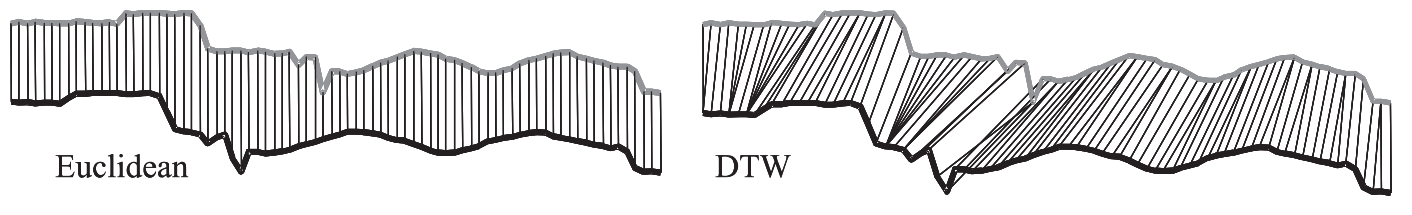
\includegraphics[width=\textwidth]{figures/EuclideanvsDTW.png}
    \caption{Comparison between a euclidean distance and a \gls{dtw} distance \cite{keogh2005exact}}
    \label{fig:euclideandtw}
\end{figure}

The standard \gls{dtw} algorithm uses dynamic programming, which fills a matrix of distance measurements and optimizes the path through it. There are also other implementations like SparseDTW or FastDTW available that require less computation time for big inputs. We decided to stay with a simple approach, since we already condensed the feature vectors to relatively small sized and the dynamic programming implementation is fast enough for these small inputs.

To classify the feature vectors, we implemented a \gls{knn} algorithm according to Dudani's paper on this behalf \cite{dudani1976distance}. With this algorithm, we can compare a new feature vector to all other vectors and record the distance to those vectors. We can then decide depending on the nearest neighbors, according to this distance, to which category (\ie user) the new feature vector belongs. To do this, we look at the $k$ vectors with the smallest distance to the new vector and count, which category is present most often.

To illustrate the \gls{knn} algorithm, a two dimensional example, as shown in Figure~\ref{fig:knnvisualization}, is better suited. On the left, we can see a plot of the already present data, represented as circles. These data-points are already categorized in three classes, shown as different colors of the circles. To categorize a new data-point \textbf{x}, we can now calculate the distance of \textbf{x} to all other points via a distance measurement. The \gls{euclideandistance} for two points is plotted as arrows in this example.

\begin{figure}
    \subfloat{%
        \begin{minipage}[c][1\width]{0.5\textwidth}%
            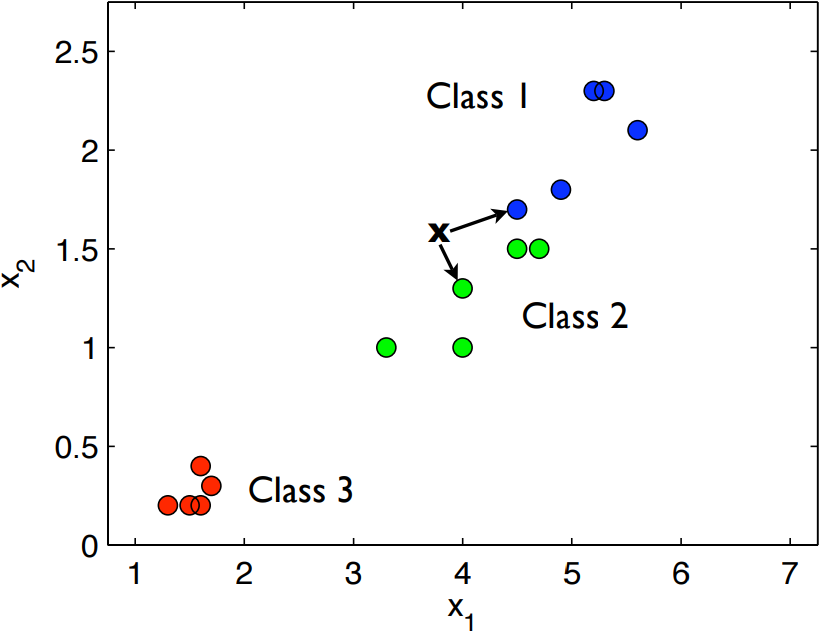
\includegraphics[width=0.99\textwidth]{figures/knnOnAxis.png}
        \end{minipage}
    }
    \subfloat{\centering{}%
        \begin{minipage}[c][1\width]{0.5\textwidth}%
            \centering
            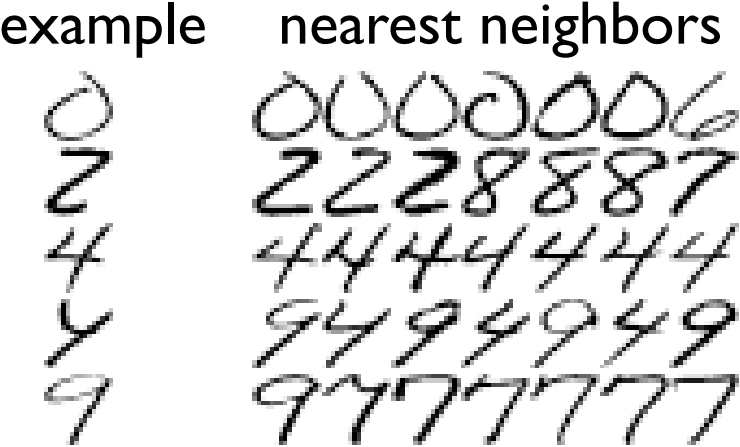
\includegraphics[width=0.99\textwidth]{figures/knnNearestNeighbors.png}
        \end{minipage}
    }
    \caption{2D visualization of the \gls{knn} algorithm. On the left: Distances between points, defining nearness to neighbors; On the right: Nearest neighbors of hand drawn digits \cite{lewick2007clustering}}
    \label{fig:knnvisualization}
\end{figure}

With the distances between the data, we can now determine the \emph{nearest neighbors}, \ie the data-pints with the smallest distance. We can then do a majority decision between the $k$-nearest neighbors, to which class the new data-point belongs. The effect of this parameter $k$ is visualized on the right side of Figure~\ref{fig:knnvisualization}. In most examples, the nearest neighbors have a strong tendency towards a class, however, in edge cases $k$ can influence the final decision towards a certain class.

In our limited test, we found, that $k = 7$ resulted in sufficiently good results. However, this parameter probably needs tuning for real applications, as the datasets might get arbitrarily large.

Another approach would be to define and train neuronal networks to classify the available data. One open source framework for neuronal networks is Encog \cite{heaton2016encog}. Due to the complexity and time requirement, this approach exceeds the scope of this Bachelor's thesis, but definitely is a promising future approach, which needs to be evaluated.

\section{Data storage and processing}
Since with recording acceleration data, we are generating many individual data sets, that need to be stored for later analysis. The lifetime of Android apps is mostly controlled by the user. Therefore, we need a way to safely and persistently store the recorded data. With this data, we can also compare different approaches in preprocessing and classification without the need to constantly interact with the device.

\subsection{SQLite Database}
To store the data on the device, we use a SQLite database. This is the standard Android SQL database for persistent storage on the device. SQLite is an extremely lightweight database with little to no additional features. Since we do not need extra database features except inserting and querying the data, SQLite is a good fit for our use case.

SQLite also stores the database in a single standardized file with a user-defined name, in our case \lstinline$SensorMeasurements.db$. This allows to share the data between devices for debugging and data visualization. In our example prototype, the database is regularly copied to a folder accessible with USB, since the usual storage of the database is inaccessible for other processes running on the device. We then can access the database copy from a connected PC, where we can visualize the algorithms directly on the data with a simple Python script.

The schema of the database is displayed in Figure~\ref{fig:dbschema}. With this schema, we are  storing the raw recorded data in so called ``datasets''. $N$ of the data points in a dataset form a whole measurement, which is linked to a single user. We also record the keystrokes in each of the measurements, when the user is using the on-screen keyboard. We then can correlate the ``sensortime'' we measured the individual acceleration in the dataset with the ``keystroketime'' to compare, if we correctly detected a keystroke. We also deduced the average keystroke and sensor-measurement frequency used in the parameters for the algorithms mentioned in the last sections.
\begin{figure}
    \centering
    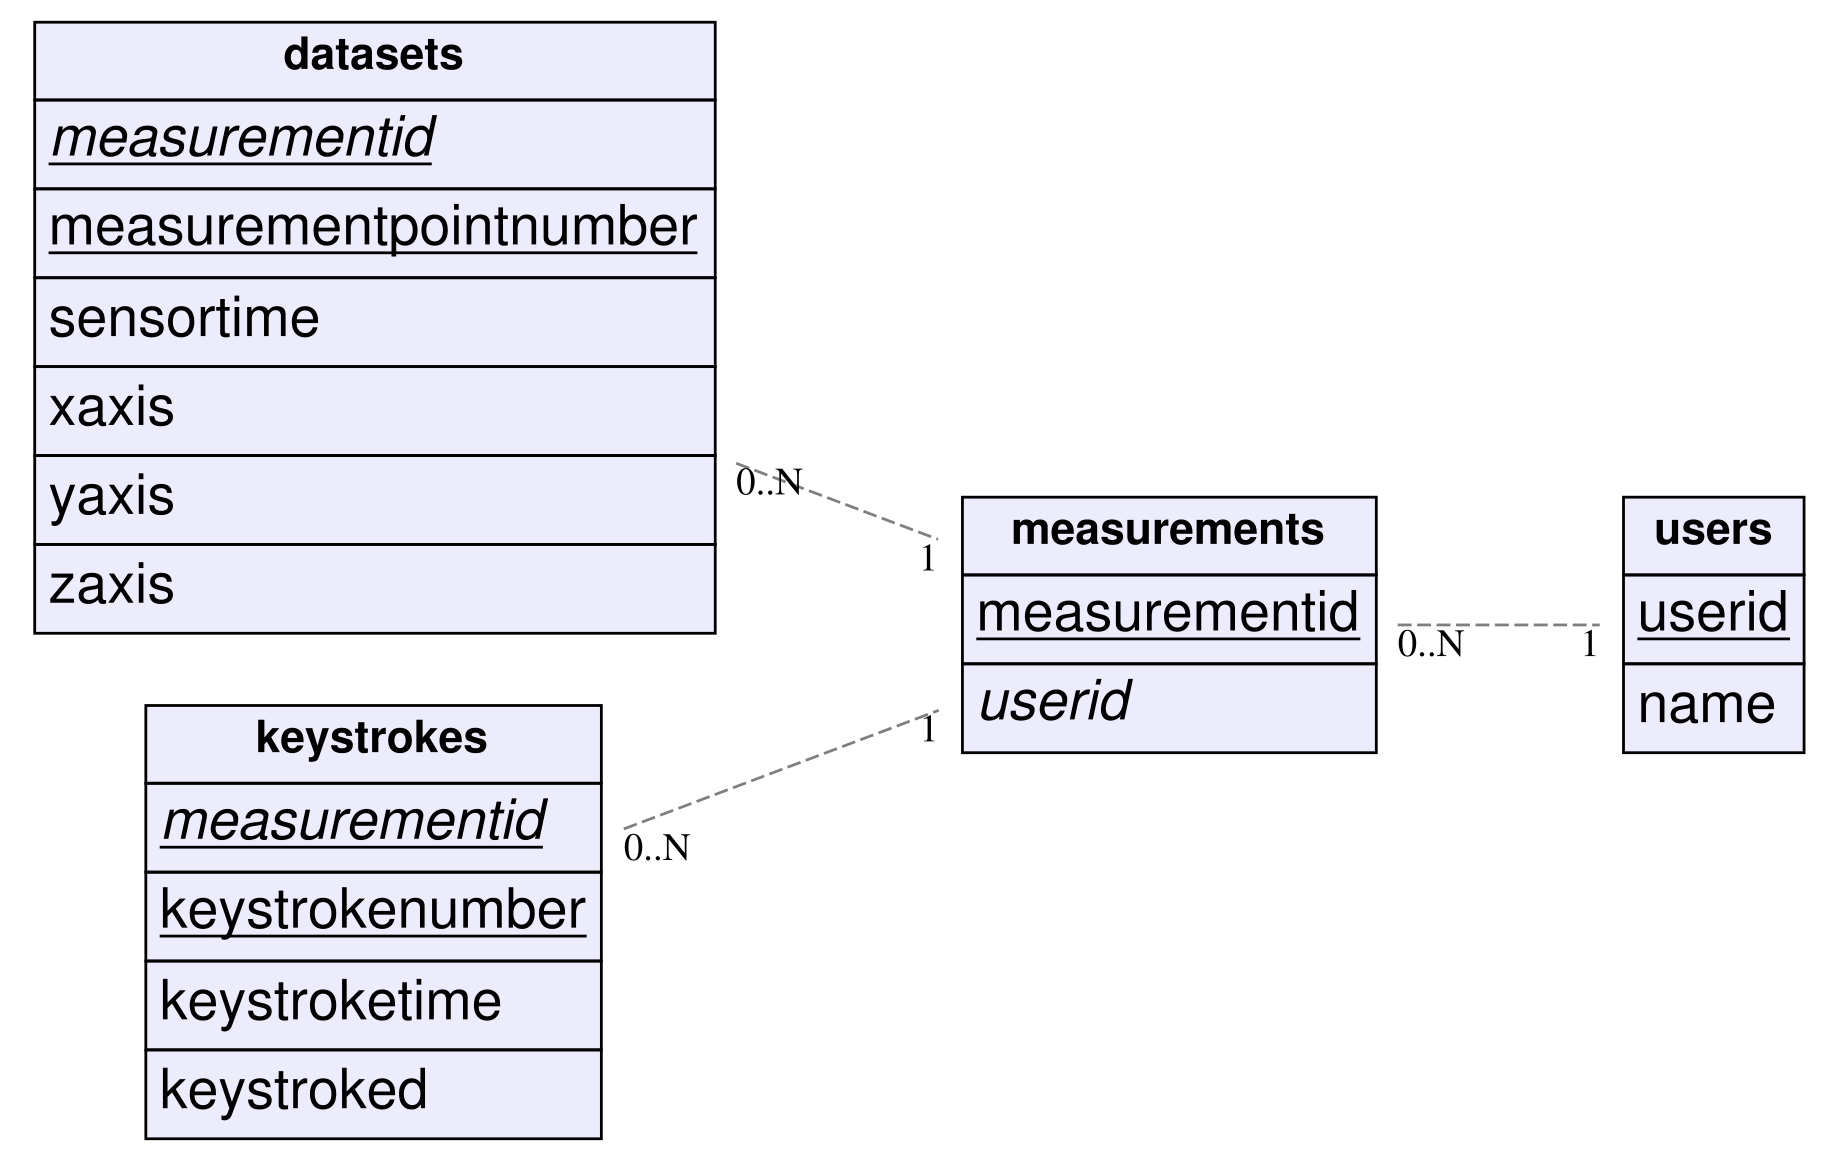
\includegraphics[width=0.93\textwidth]{figures/databaseschema.png}
    \caption{Schema of the SQLite database used by the prototypes}
    \label{fig:dbschema}
\end{figure}

\subsection{Background verification of patterns}
Since the measurement data is persistently stored, we can also implement a background verification and identification of the users. These background identity checks would allow for the benefits of the additional stronger authentication, without bothering or interrupting the user.

Currently, this is only a plan for future improvements. As of now, we only directly check the measured data. However this can easily be implemented with additional work.
\section{App prototypes}
The individual app prototypes and source code are available online via GitHub (\url{https://github.com/pfent/GesturesID}) or via the attached CD. The structure of the files is as follows: In the ``Android'' folder, there is an Android Studio project called ``GesturesID'', which contains the source code of the prototypes. In the same folder, there are also two \lstinline$.apk$ files, which can be installed on an Android, respectively an Android Wear device. This project can be built via the Android Studio \gls{ide} or via evecuting the Gradle wrapper script \lstinline$gradlew$.

The source code itself is structured in 3 different modules: \lstinline$app$: the Android specific source code; \lstinline$wear$: the Android wear specific code and \lstinline$sensorprocessing$: the code that can be used in both apps. Generally speaking, all the portable classes are located in the \lstinline$sensorprocessing$ module. This includes the implementation for recording the sensors, preprocessing, analyzing and classification. The corresponding classes are structured in loosely coupled \glspl{package}, which are accordingly named.

Additionally, the portable library module also provides a \lstinline$MeasurementManager$ for persistently storing the data. To interface with platform specific code, we also provide a Listener-interface, that is used for callbacks when a pattern has been recorded.

\subsection{Android application}
\begin{figure}
    \centering
    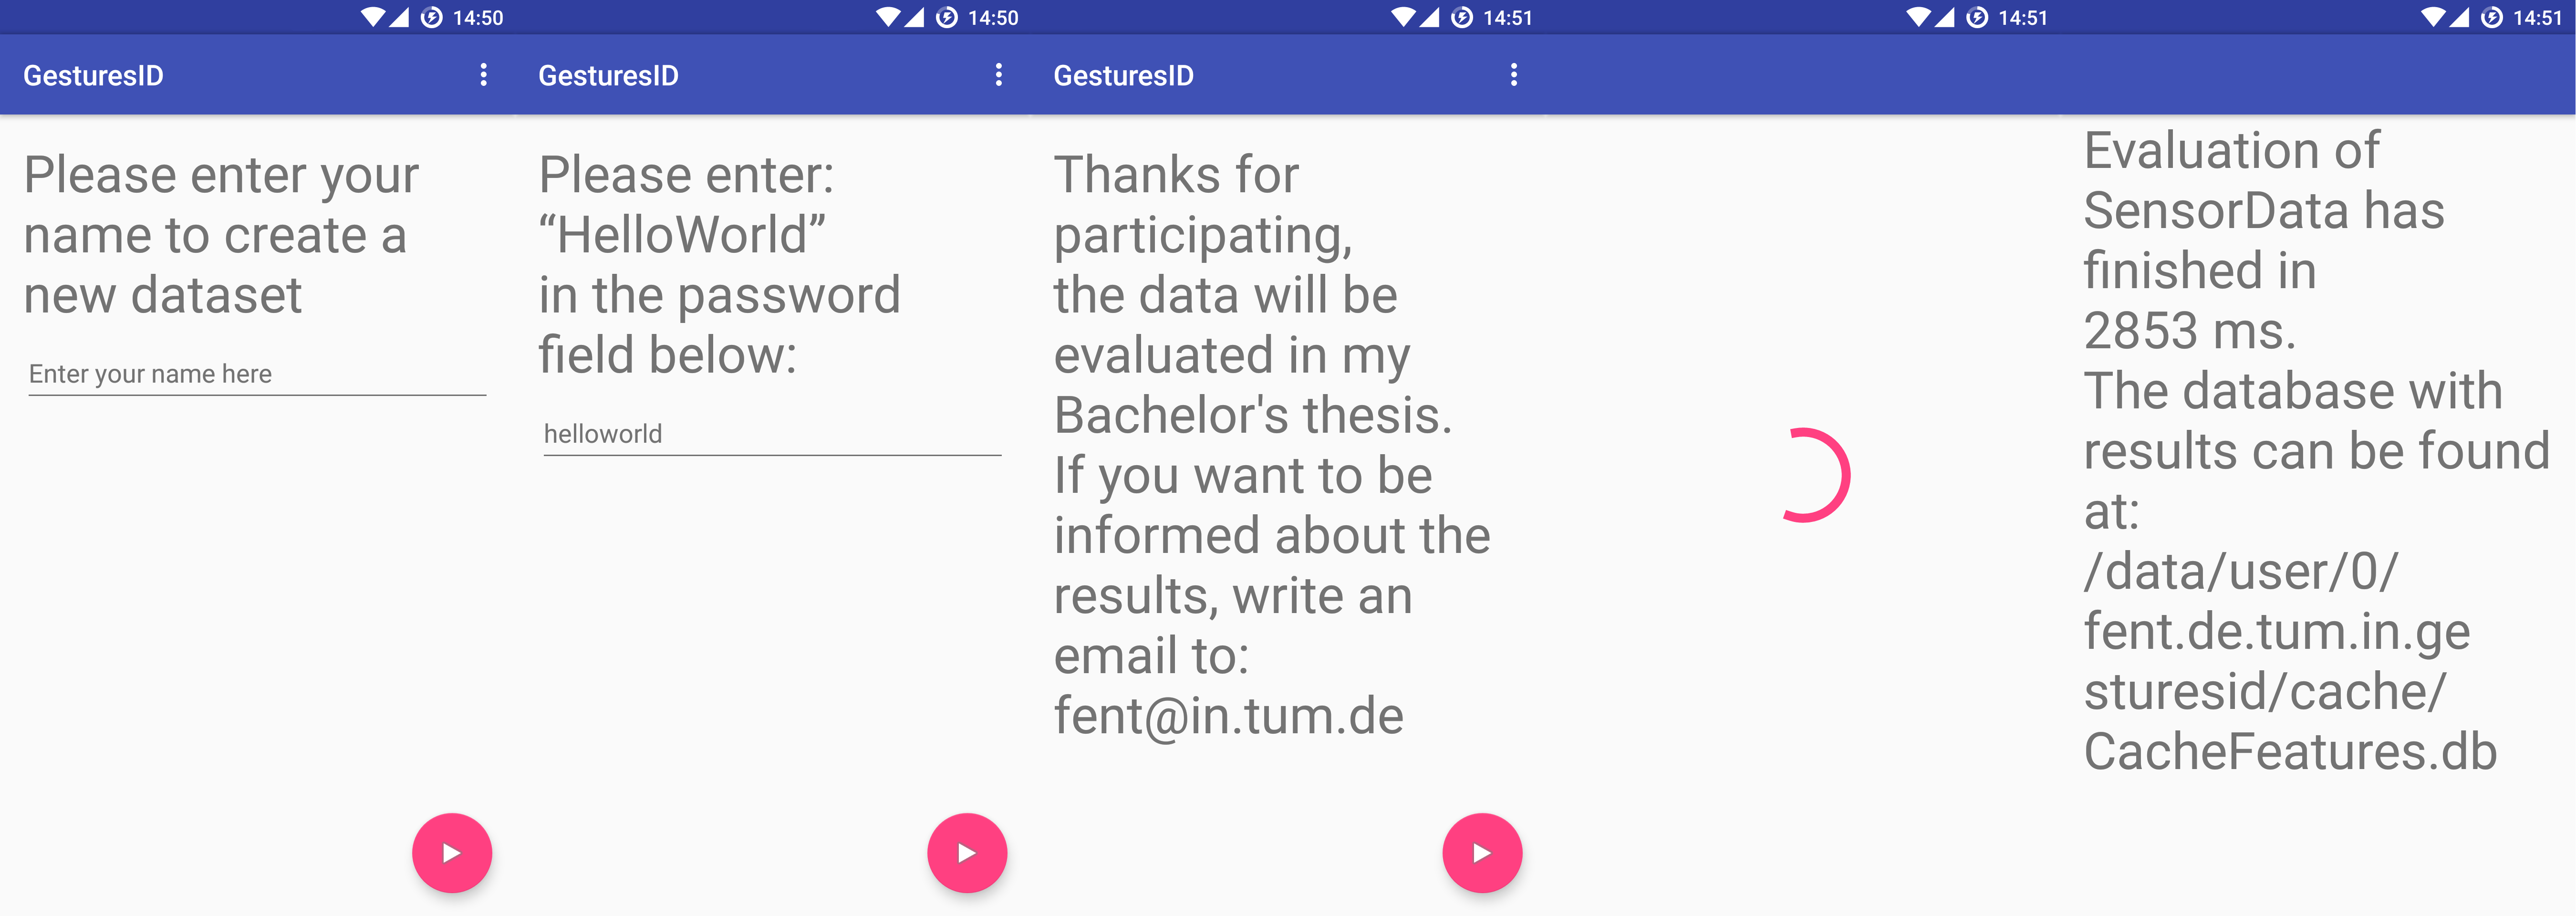
\includegraphics[width=\textwidth]{figures/MeasurementPhone.png}
    \caption{Screenshots of the prototype Android \gls{app}, in sequence of execution. The left three screenshots show the interface to enter training data, the right two screenshots, how the data is being processed}
    \label{fig:phonescreenshot}
\end{figure}

The standard Android \gls{app} provides two \glspl{activity}. Both \glspl{activity} are launchable via Android's integrated \gls{app} launcher, \ie there are two different \gls{app} icons. The first \gls{activity} ``GesturesID'' is used to create training data and only records data. This activity can be seen in the screenshots on the left of Figure~\ref{fig:phonescreenshot}.

In the current implementation, the user is first prompted to input a name, which is later used to identify the individual measurements. Afterwards, the user is prompted to enter a predefined sequence  to generate acceleration data for testing the pattern detection algorithm. The start and end of measurements is determined by a \lstinline$PatternFocusChangeListener$. This listener analyzes the ``focus'' of the user and generates events, when the user taps into the \lstinline$EditText$ component to input text. When the user taps the enter key or proceeds to the next input field, this ``focus'' is lost and the listener fires an end event and we stop recording data.

In the second \gls{activity}, the data is then processed with the algorithms described in the last sections. For the prototype, we are only using the normalized z-axis data. From this normalized data we then extract the features in a \lstinline$PhoneKeystrokeFeatureExtractor$, which first determines the peaks aka keystrokes in this data. From these peaks we then can calculate the intensity of the individual taps and the intervals, in which the keys were stroked. A small code sample, how this could be implemented using our library can be seen in Listing~\ref{lst:keystrokefeatures}.

\begin{lstlisting}[float,
caption={Minimum working example to extract keystroke features},
label={lst:keystrokefeatures}]
SensorData data = new ComposingPreprocessor(
    new Selector(2), // Select Z-Axis
    new Normalizer()
).preprocess(
    MeasurementManager.getInstance(context).getSensorData(measurementID)
);
FeatureVectors vectors = new PhoneKeystrokeFeatureExtractor().extractFeatures(data);
\end{lstlisting}

Even though, we implemented and tested smoothing of the sensor data, we found, that smoothing the measurements did not provide better keystroke recognition rates, but also decrease accuracy in the tap intensities. With further investigation, we found that smoothing the measurements is unnecessary overhead, since the peak detection algorithm is specially engineered to ignore measurement noise via the standard deviation.

After this learning phase, we then can classify new measurements, which have been processed in the same way as the training data. The classification process is displayed in Listing~\ref{lst:authenticationprocess}. For this prototype, we are using a \gls{knn} classifier with a \gls{dtw} distance measurement. The \gls{app} then displays the time used to process all of the previously recorded measurements and displays the location, where it stored the intermediate results.

\begin{lstlisting}[float,
caption={Minimum working example to classify a given \lstinline$FeatureVectors$ according to previously learened \lstinline$categories$},
label={lst:authenticationprocess}]
int classify (FeatureVectors[][] categories, FeatureVectors featureVectors)
    Classifier classifier = new kNNClassifier(categories, new dTWDistancer(3), 7);
    int category = classifier.classify(featureVectors);
    // category now contains the index of the category in categories[][], 
    // where featureVectors belongs to
    return category
}
\end{lstlisting}

\subsection{Android Wear application}
\begin{figure}
    \subfloat{%
        \begin{minipage}[c][1\width]{0.5\textwidth}%
            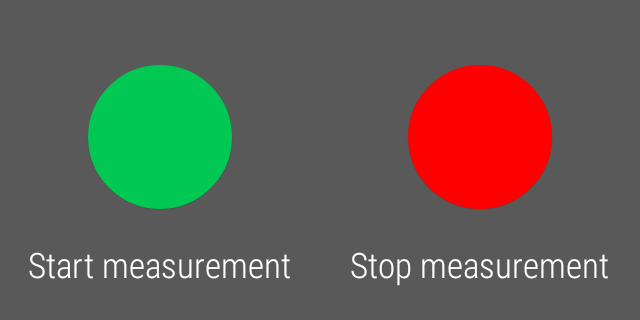
\includegraphics[width=0.999\textwidth]{figures/MeasurementWatch.png}
        \end{minipage}
    }
    \subfloat{\centering{}%
        \begin{minipage}[c][1\width]{0.5\textwidth}%
            \centering
            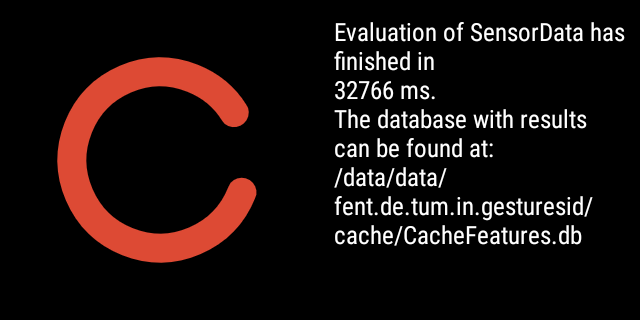
\includegraphics[width=0.999\textwidth]{figures/EvaluationWatch.png}
        \end{minipage}
    }
    \caption{Screenshots of the prototype Android Wear \gls{app}, in sequence of execution. The left two screenshots show the interface to record training data, the right two screenshots, how the data is being processed}
    \label{fig:wearscreenshots}
\end{figure}
The Android Wear \gls{app} is roughly built in the same shape as the Android \gls{app}. The \gls{app} has two launchable \glspl{activity}, one to record patterns and one to process them. However, the implementation is less sophisticated, due to time constraints. The recording of patterns is manually initiated by clicking a button, as displayed in the left half of Figure~\ref{fig:wearscreenshots}. After starting the measurement, the button turns red and the measurement can be stopped by clicking the button again.

While the Android \gls{app} can automatically associate a user with a measurement by prompting to enter a name, this is not possible on Android Wear due to the lack of text entering methods on this platform. This would be possible for example with a companion \gls{app} on a PC or on a phone, but has not been implemented yet.

The previously recorded measurements can be processed directly on the device, via the second \gls{activity}: \lstinline$EvaluationActivity$, displayed on the right half of Figure~\ref{fig:wearscreenshots}. Currently the implementation only processes the measurement in the same way as the Android \gls{app}. This might not result in the best user-detection results, but can serve as a approximate performance measurement.

\subsection{Limitations}
In the current state, both prototypes work as a proof of concept. They allow to extract data and compare different approaches and implementations of the algorithms described in Chapter~\ref{chapter:approaches}. To authenticate and validate user identities, additional work needs to be done, which can be largely based on the results of this thesis.
